\documentclass[tikz,border=5mm]{standalone}
\usepackage[utf8]{vietnam}
\usepackage{tikz,tkz-euclide}
\usetikzlibrary{calc}
\begin{document}
	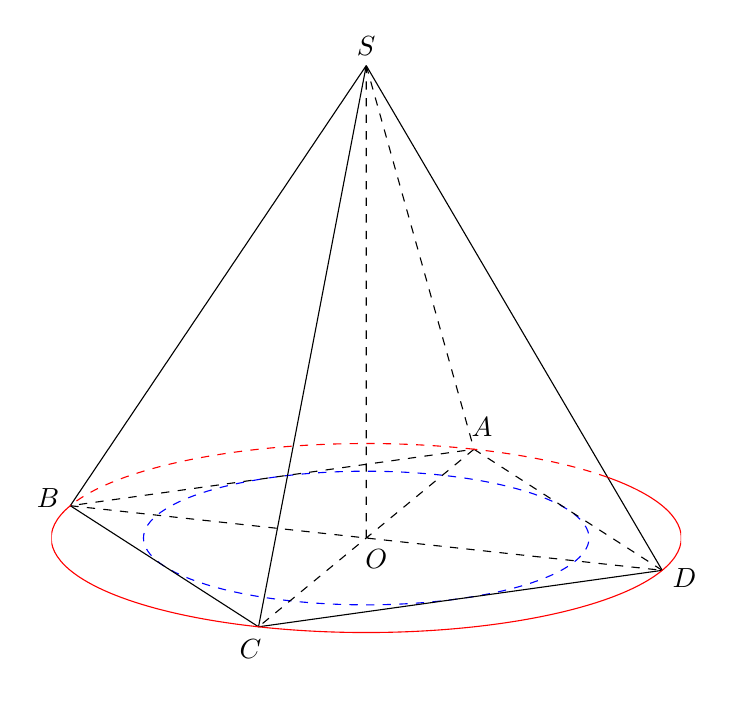
\begin{tikzpicture}
		\def\r{4} %bán kính đường tròn lớn
		\def\g{70} %góc nhìn
		\begin{scope}[yscale=0.3,rotate=\g]
			\foreach \k/\p in {0/A,1/B,2/C,3/D}
			\path (90*\k:\r) coordinate (\p) node[shift={(90*\k+\g:3mm)}] {$\p$};
			\path (0,0) coordinate (O) node[shift={(-135+\g:3mm)}] {$O$};
			\pgfmathsetmacro{\a}{\r*sin(45)}
			\draw[dashed,blue] (O) circle (\a);
			%\draw[red] (O) circle (\r);
		\end{scope}
		\path ($(O)+(0,6)$) coordinate (S) node[above] {$S$};
		\draw[dashed] (D)--(A)--(B) (A)--(C) (B)--(D) (O)--(S) (S)--(A);
		\draw (B)--(C)--(D) (S)--(B) (S)--(C) (S)--(D) ;
		\begin{scope}
			\clip (S)--(B)--(D) (-4,-2) rectangle (4,4);
			\draw[yscale=0.3,rotate=\g,red] (O) circle (\r);
		\end{scope}
		\clip (S)--(B)--(D);
		\draw[yscale=0.3,rotate=\g,red,dashed] (O) circle (\r);
	\end{tikzpicture}